\chapter{分形拓扑绝缘体}
在拓扑的十重对称性分类(表\ref{tab:tenfold})中,具有同样对称性的模型在不同的维度下可能具有不同的拓扑分类。例如$D$分类,即当模型不具有时间反演对称性(TRS)以及手性对称性(SLS),但遵守粒子空穴对称性时(PHS)。此时若系统是一维的,那么理应满足$Z_2$分类的拓扑数,若系统是二维的,则应当由$Z$分类的拓扑数描述。又或者$A$类,也即霍尔丹模型的分类,其仅在二维存在$Z$分类的拓扑数,在一维和三维没有对应的拓扑分类。

\begin{table}[h!]
\centering
\begin{tabular}{|c|c|c|c|c|c|c|}
\hline
Class & TRS & PHS & SLS & $d=1$ & $d=2$ & $d=3$ \\ \hline
A (unitary) & $0$ & $0$ & $0$ & $-$ & $\mathbb{Z}$ & $-$ \\ \hline
AI (orthogonal) & $+1$ & $0$ & $0$ & $-$ & $-$ & $-$ \\ \hline
AII (symplectic) & $-1$ & $0$ & $0$ & $-$ & $\mathbb{Z}_2$ & $\mathbb{Z}_2$ \\ \hline
AIII (chiral unitary) & $0$ & $0$ & $1$ & $\mathbb{Z}$ & $-$ & $\mathbb{Z}$ \\ \hline
BDI (chiral orthogonal) & $+1$ & $+1$ & $1$ & $\mathbb{Z}$ & $-$ & $-$ \\ \hline
CII (chiral symplectic) & $-1$ & $-1$ & $1$ & $\mathbb{Z}$ & $-$ & $\mathbb{Z}_2$ \\ \hline
D & $0$ & $+1$ & $0$ & $\mathbb{Z}_2$ & $\mathbb{Z}$ & $-$ \\ \hline
C & $0$ & $-1$ & $0$ & $-$ & $\mathbb{Z}$ & $-$ \\ \hline
DIII & $-1$ & $+1$ & $1$ & $\mathbb{Z}_2$ & $\mathbb{Z}_2$ & $\mathbb{Z}$ \\ \hline
CI & $+1$ & $-1$ & $1$ & $-$ & $-$ & $-$ \\ \hline
\end{tabular}
\caption{拓扑的十重对称分类}
\label{tab:tenfold}
\end{table}

分形几何是数学上的重要概念,其具有分数维度。在分数维度探索拓扑效应成为了一个重要的问题。以$A$类为例,一旦晶格的维度从二维降低,降低到一维是一定不存在拓扑现象,但在这之间的分数维度中,是否仍存在拓扑效应,以及这些拓扑现象会在哪个维度被截断,成为了一个有趣的问题。
\section{分形}
分形现象在自然界中普遍存在。图\ref{fig:CommonFtactal}展示了一些常见的分形示例,雪花、花椰菜和海岸线都属于分形几何的一种。尽管分形在大约400年前就开始被研究,术语“分形”(Fractal)由曼德布罗特(Mandelbrot)于1975年才首次提出\cite{mandelbrot1975fractals},来源于拉丁语“Fractus”,其原意为破碎或不规则。迄今为止,分形尚未形成统一的严格定义,通常被描述为由在某些方面与整体相似的部分构成的图形。分形具有独特的几何特性,包括非线性、不连续性和不可导性。在放大分形结构时,其局部细节与整体保持相似,体现出自相似性和尺度不变性\cite{Mandelbrot1982}。此外,分形的一个重要特征是其拥有非整数维度(分数维度)。以著名的谢尔宾斯基地毯(Sierpinski carpet)为例,当其边长放大三倍时,面积增至八倍,对应的豪斯多夫维度为 $\log_3 8 \approx 1.8928$。

\begin{figure}[htbp]
    \centering
    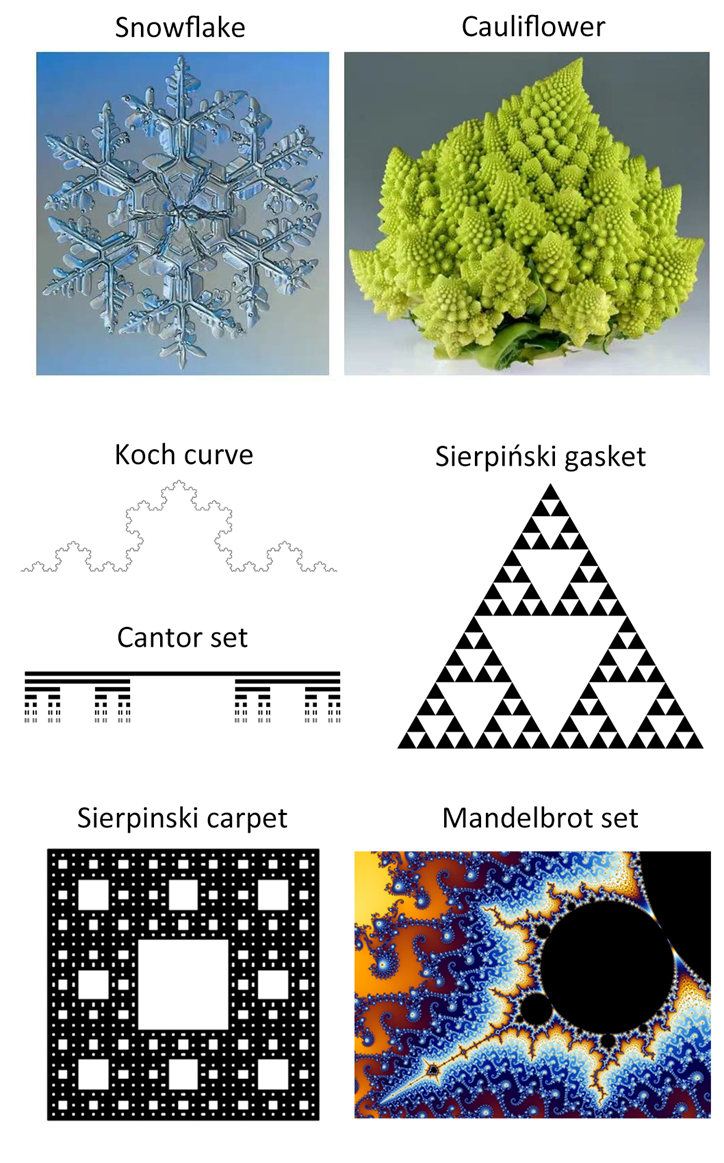
\includegraphics[width=0.5\linewidth]{FractalTopo/CommonFtactal.png}
    \caption{常见分形几何}
    \label{fig:CommonFtactal}
\end{figure}

分形的研究历史可以追溯到17世纪,莱布尼茨(Leibniz)在其著作中提出了“分形指数”的概念。随后,魏尔斯特拉斯(Weierstrass)、康托尔(Cantor)、科赫(Koch)和豪斯多夫(Hausdorff)等科学家提出了一系列经典的分形模型(图\ref{fig:CommonFtactal}),推动了分形理论的发展。1967年,曼德布罗特在《Science》杂志上发表了题为“How long is the coast of Britain? Statistical self-similarity and fractional dimension”的论文\cite{mandelbrot1967coast},并于1975年正式引入“分形”这一术语\cite{mandelbrot1975fractals}。1977年,曼德布罗特发表了《Fractals: Form, Chance and Dimension》一文\cite{mandelbrot1977fractals},标志着分形几何成为一个新的研究方向。然而,分形在随后几年内并未引起广泛关注,直到1982年第二版《The Fractal Geometry of Nature》出版后\cite{Mandelbrot1982},分形理论才逐渐受到更多科学家的重视。同年,Dan Shechtman发现了准晶材料\cite{shechtman1984metallic},并于2011年荣获诺贝尔化学奖。由于其独特的几何结构,分形与准晶在过去四十年中吸引了凝聚态物理和光学等多个领域的广泛关注。

\subsection{自相似性}
自相似性是分形几何的核心特性之一,它描述了对象在不同尺度上的重复特征。换句话说,一个自相似的分形在任意放大或缩小的尺度下都呈现出与整体相似的结构。通过这种属性,自相似性为分形的生成与研究提供了理论框架。自相似性通常可以分为三种主要类型:精确自相似性(Exact Self-Similarity),统计自相似性(Statistical Self-Similarity)和准自相似性(Quasi Self-Similarity)。

精确自相似性是分形中最严格的一种形式,其特征在于分形的某一部分与整体在几何结构上完全相同。这种自相似性曼德布罗特\cite{Mandelbrot1982}在研究分形几何时首次系统化提出,并广泛应用于诸如康托尔集(Cantor Set)\cite{georg1883uber}和科赫曲线(Koch Curve)\cite{koch1904courbe}等数学分形模型的分析中。

统计自相似性则由自然科学研究中逐渐提出。例如,地形地貌和河流网络中的统计相似性在不同尺度上具有显著性。早期,塔玛斯·维克塞克(Tamás Vicsek)在研究复杂系统时对统计自相似性做出了重要阐释\cite{barabasi1991multifractality}。

准自相似性介于上述两者之间。它描述了一种非严格意义上的相似,局部结构与整体可能不完全一致,但具有某种特征性的重复模式,最典型的例子是曼德布洛特集(Mandelbrot set)和龙形曲线(Dragon Curve)。它们满足准自相似性,因为在任意小的尺度上都可以找到与自身略有不同的小版本。

在数学上,分形可以使用迭代函数系统(Iterated Function Systems, IFS)建模。IFS定义了一组仿射变换函数,每个函数将原始分形的一部分映射到更小的子区域。通过不断迭代这些变换,可以生成具有自相似性的几何图形。一个典型的例子是科赫曲线(Koch Curve)\cite{koch1904courbe},见图\ref{fig:CommonFtactal}。其通过以下规则生成:将一条线段分为三部分;用等边三角形的两条边替代中间部分;对每个新生成的线段重复上述过程。通过这种递归过程,科赫曲线在每一级迭代中都保留了与整体类似的特征,从而展示了其精确自相似性。

由于自相似性广泛存在于自然界与人造系统中,它在多个领域具有重要的应用。在自然科学中,研究树木、血管、地形等自然系统的分形结构,例如Fournier等人在1982年提出了分形算法用于模拟地形生成。他们使用统计自相似性来创建真实感的地形图,这是分形在计算机图形学领域的一个重要应用\cite{fournier1982computer}。Aristid Lindenmayer 的 L-System 是一种基于自相似性生成植物生长模式的形式语言,用于模拟植物的生长和分枝结构。这在计算机图形学和生物学中都得到了广泛应用\cite{lindenmayer1968mathematical}。在计算机科学中,自相似性被用在图像压缩算法中。E. Jacquin 在 1992 年提出了分形图像编码方法,其核心思想基于自相似性,通过在图像中寻找相似的子块,用数学方式记录下这些相似性以进行压缩\cite{jacquin1992image}。在物理学中,自相似性被用于湍流研究。自相似性可用于描述能量分布的多尺度特性,例如在复杂动力学系统中的相关应用\cite{feder2013fractals}。综上所述,自相似性不仅为人类理解复杂系统提供了一个新视角,也启发了众多工程领域的技术革新。

\subsection{分数维度}
分数维度(Fractional Dimension),又称为分形维度(Fractal Dimension),是分形几何中最重要的特征之一,用于定量描述分形结构的复杂性。传统的欧几里得几何使用整数维度(如1维的线、2维的面和3维的体)描述形状。然而,对于自然界中的许多复杂对象,如海岸线、云、河流网络、植物叶脉结构等,这些几何维度显然不足以准确反映其形态特征。

\begin{figure}[htbp]
    \centering
    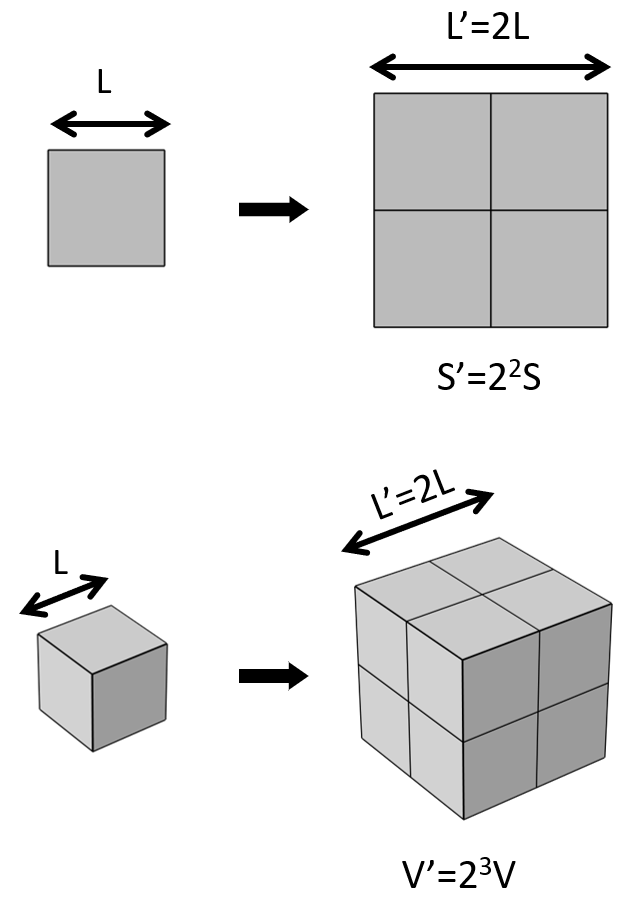
\includegraphics[width=0.3\linewidth]{figure/FractalTopo/Dimension.png}
    \caption{维度示意图}二维平面经过边长加倍后,其面积变为原来的$2^2$倍;而三维正方体经过边长加倍后,其体积变为原来的$2^2$倍。可以发现其面积(体积)加倍的指数项就是几何的维度。
    \label{fig:enter-label}
\end{figure}

分数维度这一概念虽然在数学中由来已久,但这个术语本身是由本华·曼德布洛特在1967 年关于自相似的论文中提出的\cite{mandelbrot1967coast}。通过引入非整数维数的概念,提供了一种更为灵活的方法来描述这些复杂结构的形态特征 \cite{Mandelbrot1982,falconer2013fractal}。计算分形维度的方法有很多,例如信息维度、关联维数、广义维数、樋口维数、李雅普诺夫维数等。本节将介绍最经典的两种维度计算方式:Hausdorff维度和盒计数维度。

\subsubsection{Hausdorff维度}
Hausdorff维度是分形几何中一种严格定义的分数维度,用于描述集合的复杂性。它以数学上的Hausdorff测度(Hausdorff measure)为基础定义,是度量空间中集合复杂性和细节丰富程度的一种刻画。

Hausdorff维度 $d_H$ 的定义依赖于Hausdorff测度。给定一个集合 $S \subset \mathbb{R}^n$ 和一个正数 $s$,其Hausdorff测度 $H^s(S)$ 定义为:
\begin{equation}
    H^s(S) = \lim_{\delta \to 0} \inf \left\{ \sum_i \text{diam}(U_i)^s \right\},
\end{equation}
其中,$\{U_i\}$ 是一个覆盖集合 $S$ 的开集家族,满足 $S \subseteq \bigcup_i U_i$;$\text{diam}(U_i)$ 表示覆盖集 $U_i$ 的直径,即 $\text{diam}(U_i) = \sup\{d(x, y) : x, y \in U_i\}$;$\delta > 0$ 是覆盖集中每个 $U_i$ 的直径上限。

Hausdorff维度 $d_H$ 定义为使得 $H^s(S)$ 在 $s$ 维度转变时从无穷到零的临界值:
\begin{equation}
d_H = \inf \left\{ s : H^s(S) = 0 \right\}.
\end{equation}
简单来说,Hausdorff维度描述了覆盖分形集的度量空间中的最小球体的直径和数量之间的关系,因此可以精确描述分形的尺度不变性。Hausdorff维度测量的是一个集合在不同尺度下的复杂性。它通过将集合分解为更小的覆盖单元,观察这些单元的尺寸如何随着分辨率的改变而变化,从而描述集合填充空间的能力。对于经典几何对象,Hausdorff维度与其欧几里得维度一致,但对于分形集合,Hausdorff维度通常是非整数。

三分之一Cantor集是一个经典分形(见图\ref{fig:CommonFtactal},Contor Set),通过以下迭代过程构造:起始时,从 $[0, 1]$ 的闭区间开始;在每次迭代中,将当前每个区间的中间三分之一去掉;无限迭代后,剩下的点集称为Cantor集。每次迭代后,剩余的区间数为 $N = 2^k$,区间长度为 $l = (1/3)^k$,其中 $k$ 是迭代次数。Cantor集是自相似的,其相似性比率为 $r = 1/3$,因此总的覆盖关系为:
\begin{equation}
    N \cdot r^s = 1,
\end{equation}
即,$2 \cdot \left(\frac{1}{3}\right)^s = 1$。解方程可得三分之一Cantor集的Hausdorff维度为$s = \frac{\log(2)}{\log(3)}$。这表明Cantor集虽然在欧几里得意义下是一维的线段(从 $[0,1]$ 的区间中构造),但其复杂性不足以填满整个一维空间,因此其维度是一个介于0和1之间的非整数值。
 
对于分形集合,如Cantor集、Sierpiński三角形等,Hausdorff维度能够有效地描述其复杂性。表\ref{tab:FracDim}展示了常见分形的Hausdorff维度。

\begin{table}[h!]
\centering
\begin{tabular}{|c|c|c|c|}
\toprule
\textbf{分形名称} & \textbf{Hausdorff 维度} & \textbf{分形名称} & \textbf{Hausdorff 维度}\\
\midrule
康托尔集 & 0.6309 & 科赫曲线 & 1.2619\\
闵可夫斯基曲线 & 1.3652 & 维切克分形 & 1.4649\\
谢尔宾斯基三角 & 1.5850 & 谢尔宾斯基六边形 & 1.6309\\
斐波纳契分形 & 1.6379 & 谢尔宾斯基正方形 & 1.8928\\
康托尔尘埃 & 1.8928 & 曼德尔布罗特集 & 2\\
佩亚诺曲线 & 2 & 谢尔宾斯基四面体 & 2\\
分形金字塔 & 2.3219 & 门格尔海绵 & 2.7268\\
\bottomrule
\end{tabular}
\caption{常见分形的 Hausdorff 维度}
\label{tab:FracDim}
\end{table}

Hausdorff维度是分形几何的核心工具,用于严格定义分数维度,量化集合在空间中的复杂性。通过Cantor集的例子可以看出,其计算依赖于集合的自相似性和覆盖尺度的变化。Hausdorff维度不仅在数学上具有深刻意义,还广泛应用于自然现象的建模和复杂系统的分析中。

\subsubsection{盒计数维度}
盒计数维度(Box-Counting Dimension)是一种常用的分形维度估计方法,因其简单易用且适合计算机实现而广泛应用。它通过研究对象在不同尺度下的覆盖情况,定量描述对象的复杂性和自相似性。
设 $S \subset \mathbb{R}^n$ 是一个有限或无限的点集,将 $S$ 用一系列边长为 $\epsilon$ 的盒子覆盖。盒计数维度 $d_B$ 定义为:
\begin{equation}
d_B = \lim_{\epsilon \to 0} \frac{\log N(\epsilon)}{\log(1/\epsilon)},
\label{eq:BoxCount}
\end{equation}
其中,$N(\epsilon)$ 是边长为 $\epsilon$ 的盒子覆盖 $S$ 所需的最小盒子数;$\epsilon$ 是盒子的边长;取极限 $\epsilon \to 0$ 表示盒子的边长无限趋于零。盒计数维度通过将对象 $S$ 放置在一个规则网格上,计算对象被覆盖所需的小网格单元(即盒子)的数量 $N(\epsilon)$ 来估计维度。盒计数维度反映了对象在空间中分布的复杂性。对于简单几何形状,盒计数维度与其欧几里得维度一致,但对于分形对象,盒计数维度通常是非整数。

本节继续以Cantor集为例。假设将 Cantor集放置在边长为 $\epsilon$ 的规则网格中。Cantor集的每次迭代产生的线段长度为 $l_k = \left(\frac{1}{3}\right)^k$,因此网格的边长选择为 $\epsilon = l_k = \left(\frac{1}{3}\right)^k$,其中 $k$ 是迭代次数。第 $k$ 次迭代时,Cantor集的剩余区间数量为 $N_k = 2^k$,即覆盖 Cantor集所需的盒子数。将 $N(\epsilon)$ 和 $\epsilon$ 代入公式\ref{eq:BoxCount}可得
\begin{equation}
d_B = \lim_{k \to \infty} \frac{k \log(2)}{-k \log(3)} = \frac{\log(2)}{\log(3)}.
\end{equation}
因此,中间三分之一Cantor集的盒计数维度为$d_B = \frac{\log(2)}{\log(3)} \approx 0.6309$。该结果与Hausdorff维度一致。

盒计数维度是一种常用的分形维度计算方法,它通过研究对象在不同尺度下的覆盖情况,提供了一种简单而有效的工具来量化复杂系统的自相似性。相较于Hausdorff维度,盒计数维度的优点在于其算法简单,易于实现。使用该方法可以对复杂的随机分形进行维度计算,例如海岸线、河流网络或植物叶片的维度\cite{Mandelbrot1982}。但其限制在于其有较强分辨率依赖,盒子的大小会影响计算结果。这导致对高维数据的计算较为复杂并且可能存在数值误差。尽管如此,由于盒计数维度可以计算自然界复杂现象的维度,并对随机分形的发展重要支持,盒计数维度成为了最普遍的维度计算方法之一。
\subsection{随机分形}
随机分形是一类通过随机过程生成的分形结构。与确定性分形不同,随机分形在生成规则中引入了概率或噪声,从而生成更接近自然现象的复杂结构。确定性分形通常无法在现实中看到,但随机分形广泛的出现于现实生活中。地形的高度变化、云的形态、河流网络的分布以及金融市场的波动等,都属于随机分形的范畴。

\begin{figure}[htbp]
    \centering
    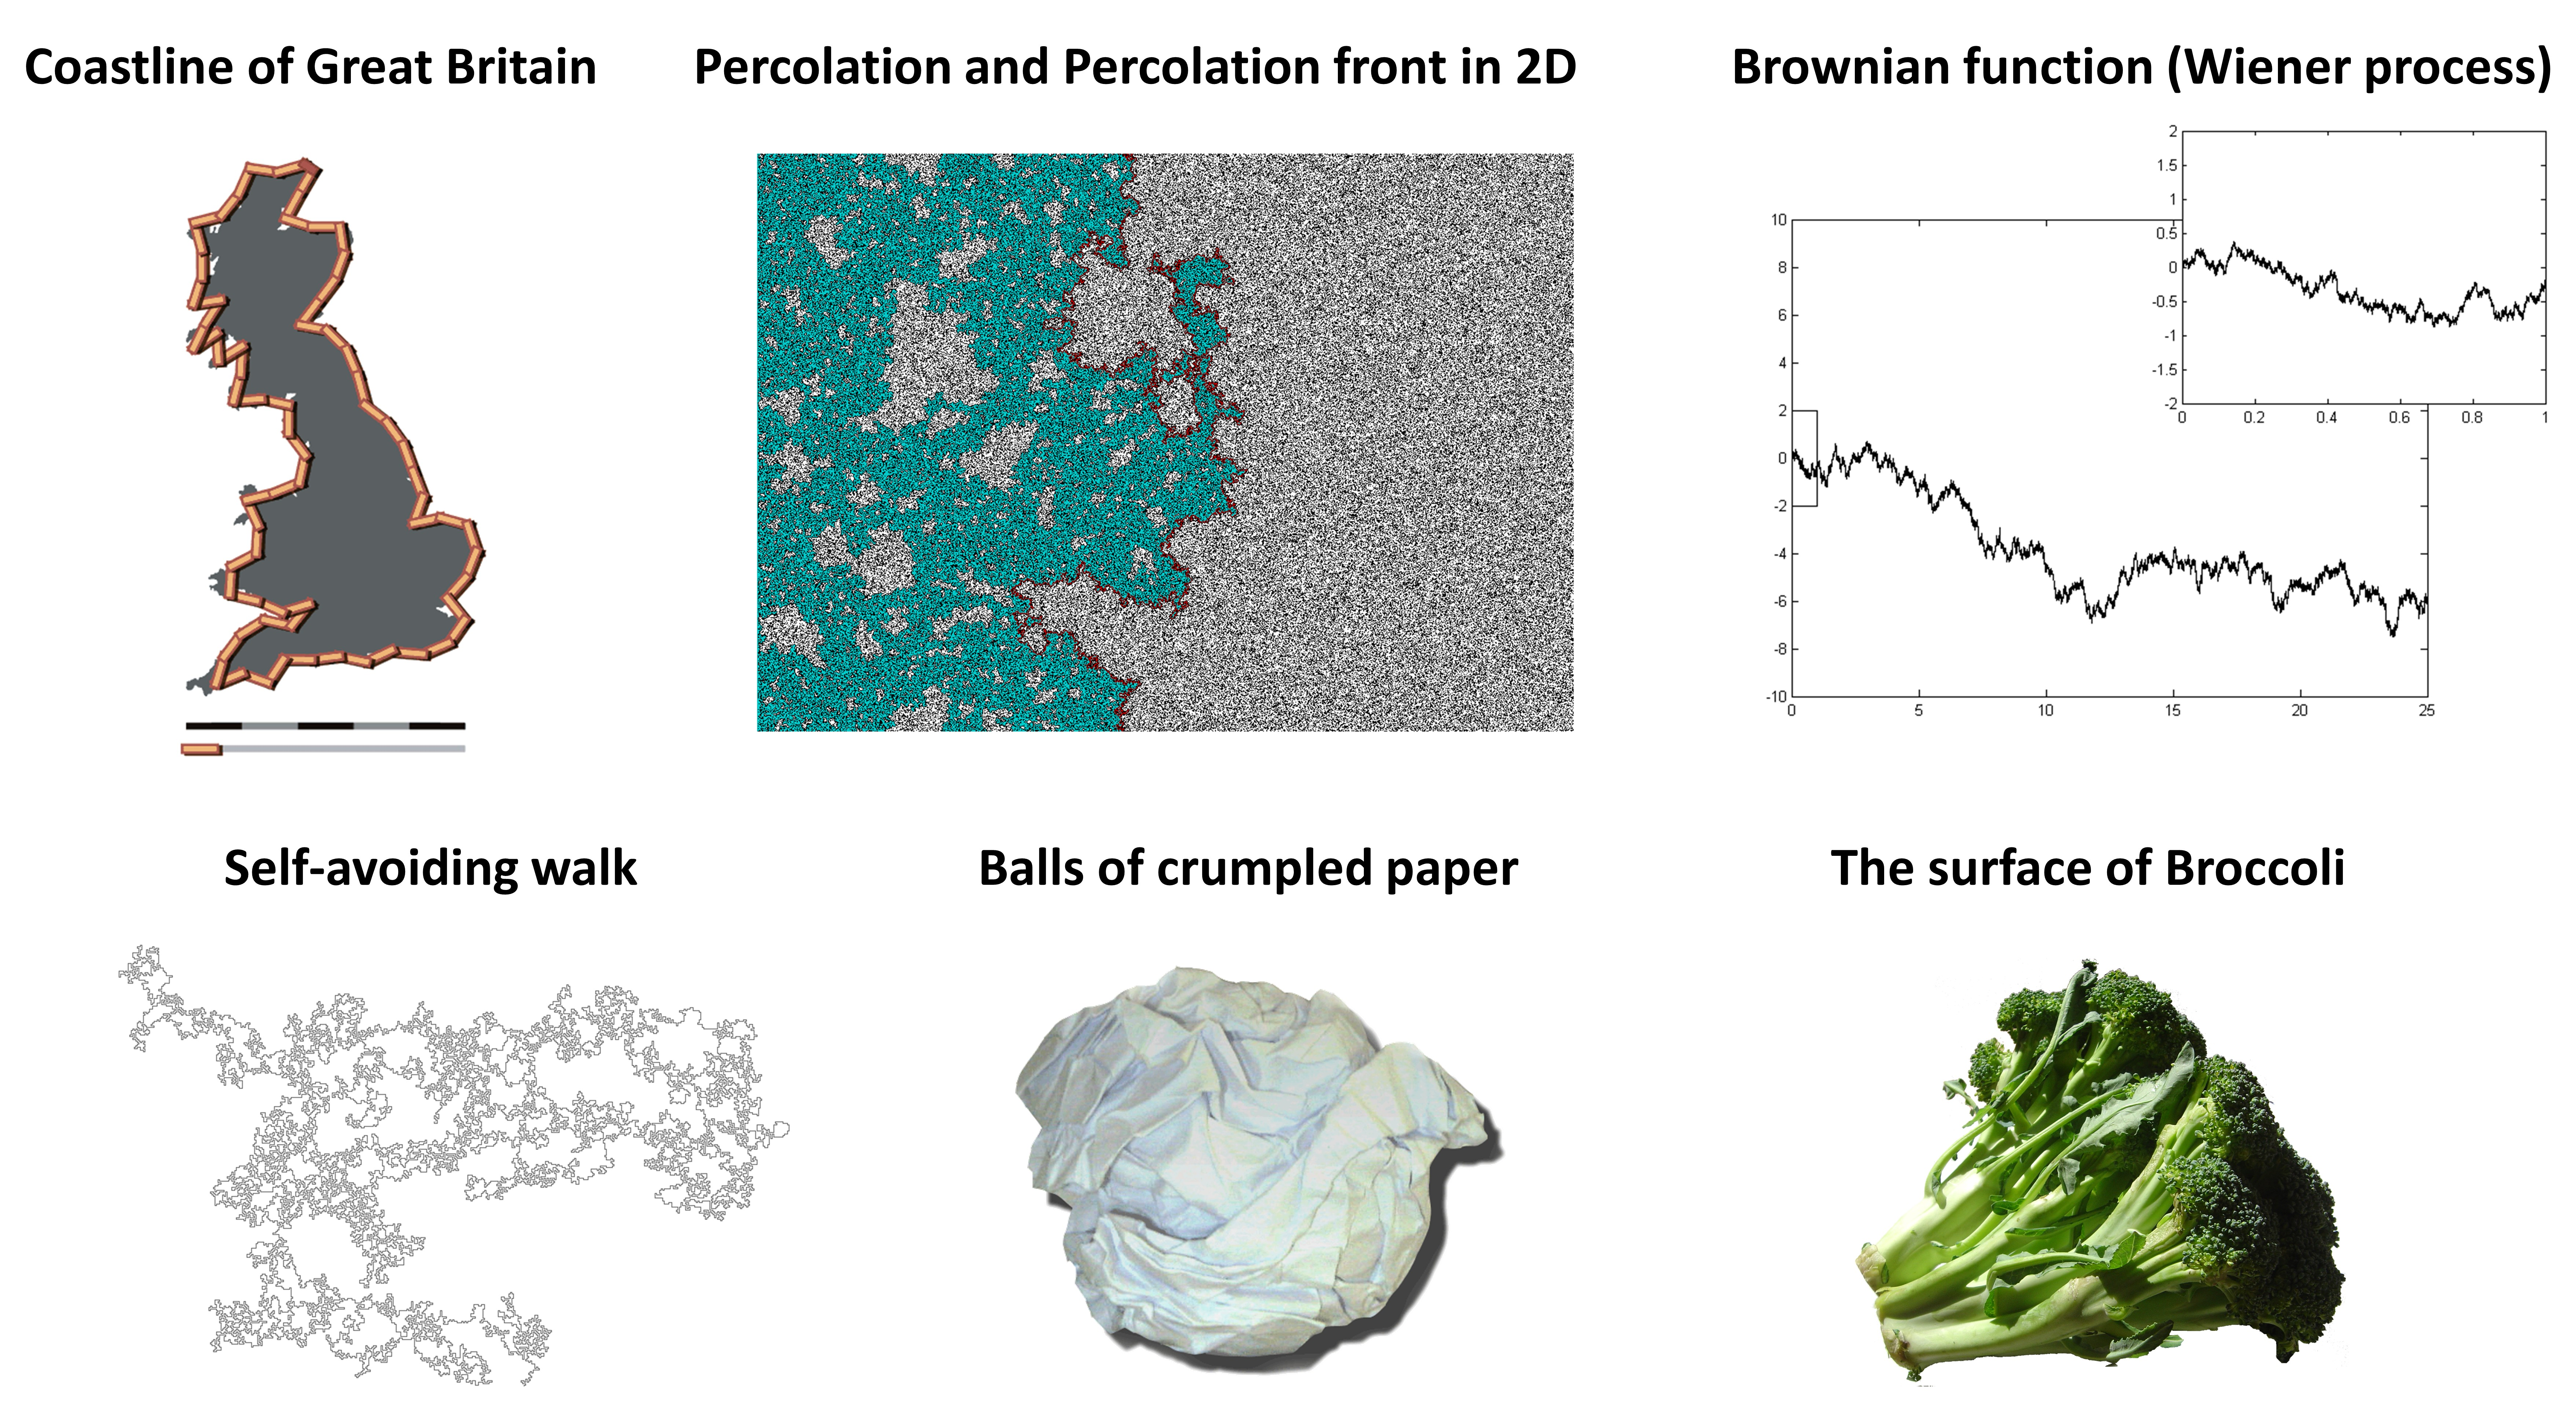
\includegraphics[width=1\linewidth]{FractalTopo/RandomFractal.jpg}
    \caption{随机分形}一系列随机分形,包括英国海岸线、渗透以及渗透前沿、布朗函数(维纳过程)、自避免的随机行走、纸团和西兰花表面。图片来源于\cite{wikipedia_hausdorff_fractals}。
    \label{fig:RandomFractal}
\end{figure}

图\ref{fig:RandomFractal}展示了一系列随机分形。图中的英国海岸线是最经典的随机分形模型之一,其引发了“海岸线悖论”,即即陆地的海岸线没有明确的长度,越来越精细的测量并不能提高精度,而只是增加了总数。Mandelbrot其在论文\cite{mandelbrot1967coast}详细讨论。论文说明了分形维度比长度更适合来描述随机分形,并给出了英国海岸线的分形维度1.25。

随机分形可以在各种日常生活中见到,例如卷起来的废纸团分形维度为2.5,花椰菜的分形维度为2.7。随机分形同样启发了很多其他领域的研究。例如在金融市场中,资产价格的变化通常是一个Weiner过程,这是一个维度为1.5的随机分形,如图\ref{fig:RandomFractal}所示,可以用布朗函数进行描述。布朗函数与伊藤引理\cite{ito1951formula}催发出的Black–Scholes公式被广泛用于对期权的定价\cite{black1973pricing}。不仅如此,在物理学中,还用于通过Fokker–Planck方程\cite{van1992stochastic}和朗之万方程\cite{langevin1908theory}研究布朗运动和其他类型的扩散。它还可以作为量子力学严格路径积分公式的基础理论\cite{kac1949distributions}以及理解宇宙学中永恒膨胀的研究。

\section{分形拓扑绝缘体的理论和实验进展}
分形结构中的拓扑物理研究可以追溯到1983年。早期研究发现,在电子分形体系中施加磁场能够产生具有自相似特性的能谱和态密度\cite{alexander1984some,banavar1985energy},但当时对分形边界上的拓扑态关注较少。2014至2015年,理论工作表明拓扑绝缘体有可能存在于准分形空间中\cite{song2014topological,he2015topological}。尽管这些研究体系并非严格意义上的分形,但其结果强烈暗示拓扑绝缘体及其边界态有望在分形晶格中实现。随着实验技术的进步,2018年在氧化铜分子的人工结构中首次实现了电子分形体系\cite{kempkes2019design},这一突破间接推动了在性能可控的人工结构中探索拓扑分形绝缘体的研究。本节将重点介绍分形拓扑物理领域在理论和实验方面的最新进展,旨在基于现有成果,为未来的研究提供参考和启示。
\subsection{分形拓扑绝缘体理论}
对于分形拓扑物理的理论研究最早可以追溯到1983年。早期研究聚焦于分形体系的能谱形状而非直接的拓扑现象\cite{alexander1984some,banavar1985energy}。而分形拓扑绝缘体的明确理论结果出现在2014年\cite{song2014topological},论文采用了Bernevig-Hughes-Zhang(BHZ)模型,
\begin{equation}
    H_{\alpha \beta}(\mathbf{k}) = 
    \begin{pmatrix}
    h(\mathbf{k}) & 0 \\
    0 & h^*(-\mathbf{k})
    \end{pmatrix}, \\
\end{equation}
非对角元为$h(\mathbf{k}) = d_0 I_{2 \times 2} + d_1 \sigma_x + d_2 \sigma_y + d_3 \sigma_z$,其中$d_0(\mathbf{k}) = C - 2D \big( 2 - \cos k_x - \cos k_y \big)$,$d_1(\mathbf{k}) = A \sin k_x, \quad d_2(\mathbf{k}) = -A \sin k_y$,$d_3(\mathbf{k}) = M - 2B \big( 2 - \cos k_x - \cos k_y \big)$。
如图\ref{fig:TopoFractal}(a)所示,作者以Koch曲线和Sierpinski地毯为例,通过计算零温条件下非平衡格林函数计算的双端导电性,研究其电子输运行为。其发现分形边界并不破坏拓扑相,拓扑边界态仍具有鲁棒性。
\begin{figure}[htbp]
    \centering
    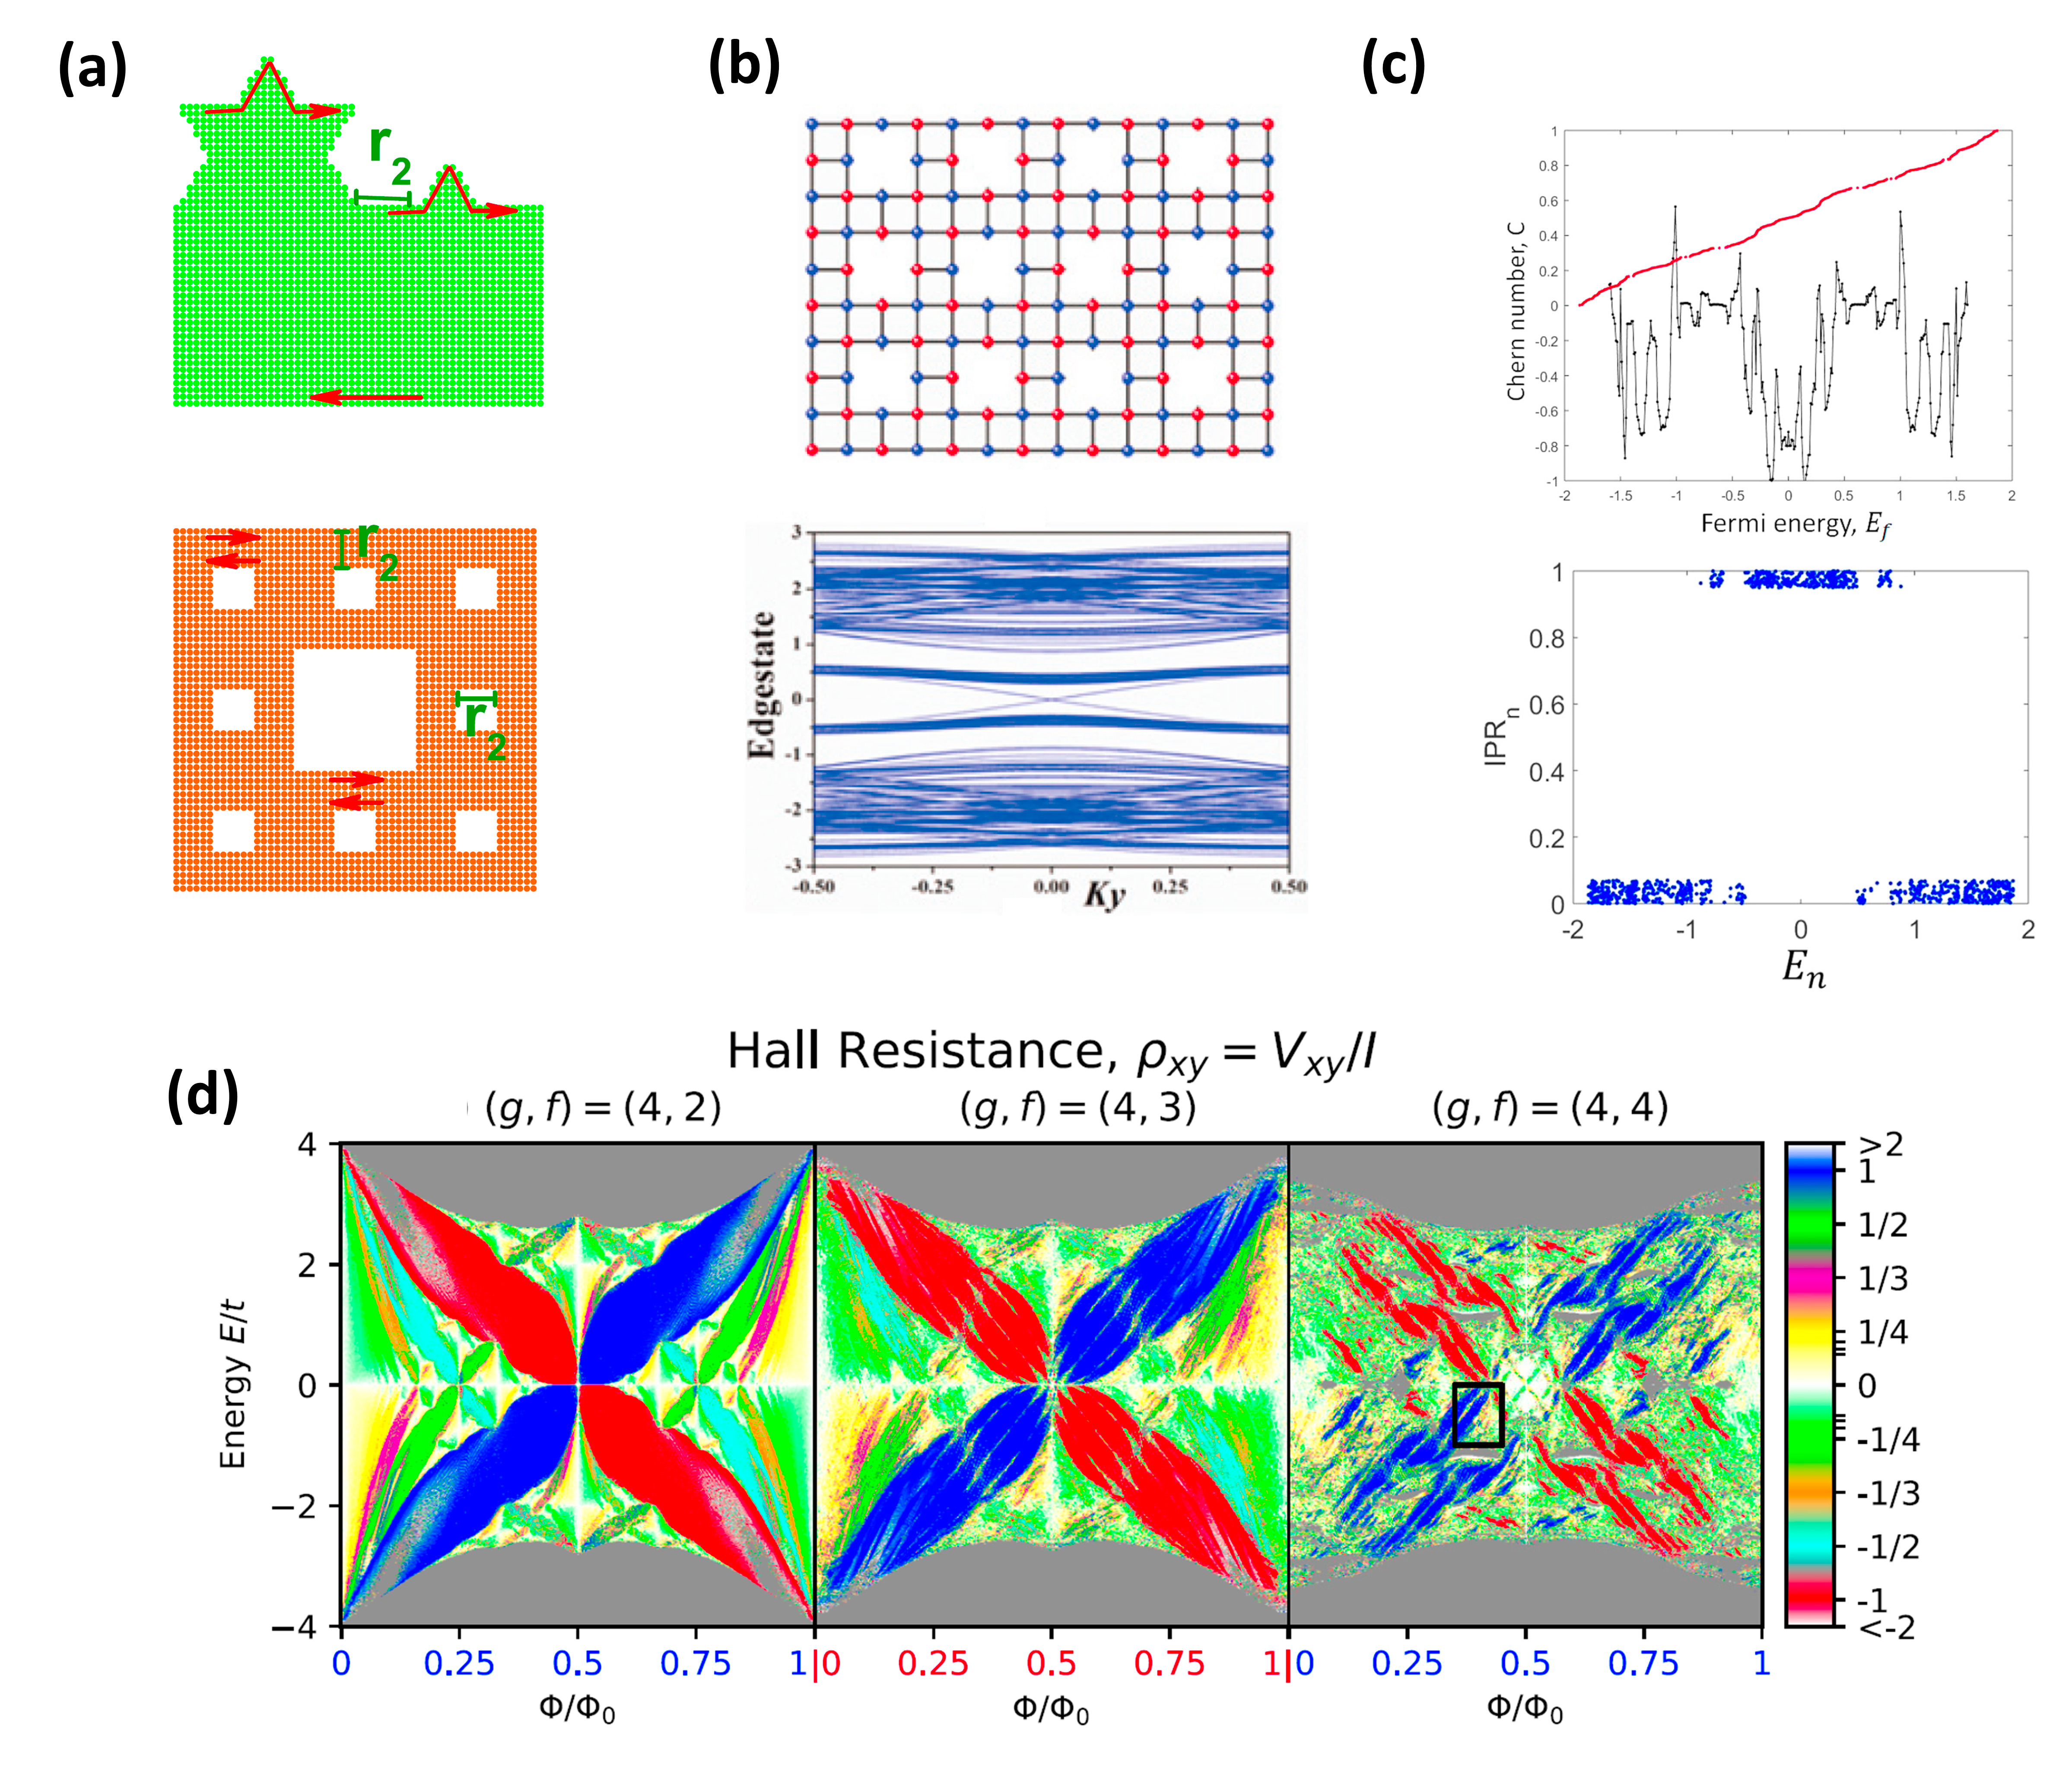
\includegraphics[width=0.6\linewidth]{figure/FractalTopo/TopoFractal.jpg}
    \caption{分形拓扑绝缘体理论进展}(a)Koch曲线和Sierpinski地毯的拓扑晶格。(b)具有自相似性空缺的分形晶格以及其能谱。(c)分形晶格的实空间陈数与逆参与比。(d)分形晶格对Hofstadter蝴蝶的影响。图片来源于文献\cite{song2014topological,he2015topological,pai2019topological,fremling2020existence}。
    \label{fig:TopoFractal}
\end{figure}
一年后,另一篇工作则计算了方晶格和蜂房晶格的Haldane模型\cite{he2015topological}。如图\ref{fig:TopoFractal}(b)所示,通过引入具有自相似性的空缺来实现分形晶格。除常规边界态外,论文发现缺陷(空位)会诱导零能态,并生成拓扑中间态(Mid-Gap States),这些在空缺里的边缘态也具有拓扑性质,受到体拓扑保护。

对于分形拓扑绝缘体的系统理论研究出现在2019年\cite{pai2019topological}。文章研究了二维无自旋的手性p-波超导体的Bogoliubov–de Gennes(BdG)哈密顿量
\begin{equation}
    H = -t \sum_{\langle r, r' \rangle} c_r^\dagger c_{r'} - \mu \sum_{r} c_r^\dagger c_r + \sum_{r, m} \left[ \Delta_m c_{r+e_m}^\dagger c_r^\dagger + h.c. \right]
\end{equation}
在Sierpinski三角形和Sierpinski地毯上的结果。除了与先前工作类似的拓扑态外,作者利用利用实空间Chern数首次计算了系统的拓扑不变量,见图\ref{fig:TopoFractal}(c)。随着分形生成代数的增加,边缘态的数量无限增多,导致谱在热力学极限下变为无隙。文章通过计算逆参与比(IPR)与能级统计表征了分形晶格上的拓扑态。在分形晶格上,拓扑态的性质受其自相似几何结构的显著影响。不同的分形结构(如Sierpinski三角形和Sierpinski地毯)可以支持无隙或有隙的拓扑相,这些拓扑相的特性与其“父晶格”上的拓扑态直接相关。该论文的研究为分形拓扑物态研究提供了理论基础,并为实验验证这些现象奠定了基础。

受到先前早期分形拓扑绝缘体工作的启发,分形晶格上的拓扑效应成为近年来理论研究的热点领域。研究者们在分形晶格上实现了多种丰富的拓扑物理现象。例如,在Sierpinski地毯结构中,分形晶格改变了霍尔电导的分布\cite{fremling2020existence, iliasov2020hall}。如图\ref{fig:TopoFractal}(d)所示,分形晶格会改变Hofstadter蝴蝶的形状。此外,高阶拓扑态的研究也取得了重要进展,例如在分形晶格中观察到了 corner states 和其他高阶拓扑现象\cite{manna2022higher,lage2024corner}。研究人员还探索了无序对分形晶格的影响,在分形系统中利用无序诱发出了安德森高阶拓扑态\cite{chen2023higher}。

在Sierpinski三角形系统中,光学实验方案的提出为分形拓扑绝缘体的实验实现提供了可能\cite{yang2020photonic}。此外,文献\cite{chen2023kitaev}解释了Sierpinski三角形中存在非整数的Chern数的原因,这为拓扑不变量的定义和理解带来了新的挑战和机遇。分形甚至可能诱发出拓扑相变,文献\cite{eek2024fractality}展示了利用各种分形晶格来诱发拓扑相变的例子和证据。

分形晶格还被用于研究相互作用系统。文献\cite{wang2022new}的研究揭示了分形晶格在相互作用系统中的拓扑序,文献\cite{jaworowski2023approximate}引入了Laughlin波函数在分形系统中的近似形式,展示了分形几何对相互作用拓扑相的影响。

除拓扑物理外,分形晶格的物理性质还在传输性质、纠缠现象、非厄米物理和相互作用系统等多个领域得到了深入研究。例如,\cite{guglielmon2019inducing, rojo2024anomalous}探讨了分形晶格中传输性质的异常表现。文献\cite{zhou2024entanglement}则研究了分形结构对量子纠缠的影响,揭示了分形几何在量子信息中的潜在应用。在非厄米物理领域,文献\cite{sun2024non,manna2023inner}的研究展示了分形晶格中非厄米系统的独特拓扑特性,分形结构中的非均匀性和自相似性为趋肤效应的产生提供了独特的条件。此外,相互作用系统还可能在分形几何背景下展现出复杂行为\cite{conte2024fractal},进一步拓宽了分形晶格研究的深度和广度。

总体而言,分形晶格上的拓扑效应研究不仅丰富了拓扑物理的理论体系,也为未来的实验实现和应用提供了广阔的前景。这些研究成果展示了分形几何与拓扑物理相结合所可能带来更多新奇物理现象和潜在技术。

\subsection{电子系统分形拓扑绝缘体}
分形晶格在电子体系有很多早期研究,最早的电子分形体系出现在2019年\cite{kempkes2019design}。通过在Cu(111)表面上精确排列CO分子,可以构建人工原子阵列,进而形成分形结构。这种方法可以用于研究电子在分形几何中的行为。作者通过扫描隧道谱测量了不同能量下的电子局域态密度,发现电子波函数在实空间和动量空间中均表现出自相似性,如图\ref{fig:ElecFractal}(a)所示。
\begin{figure}[htbp]
    \centering
    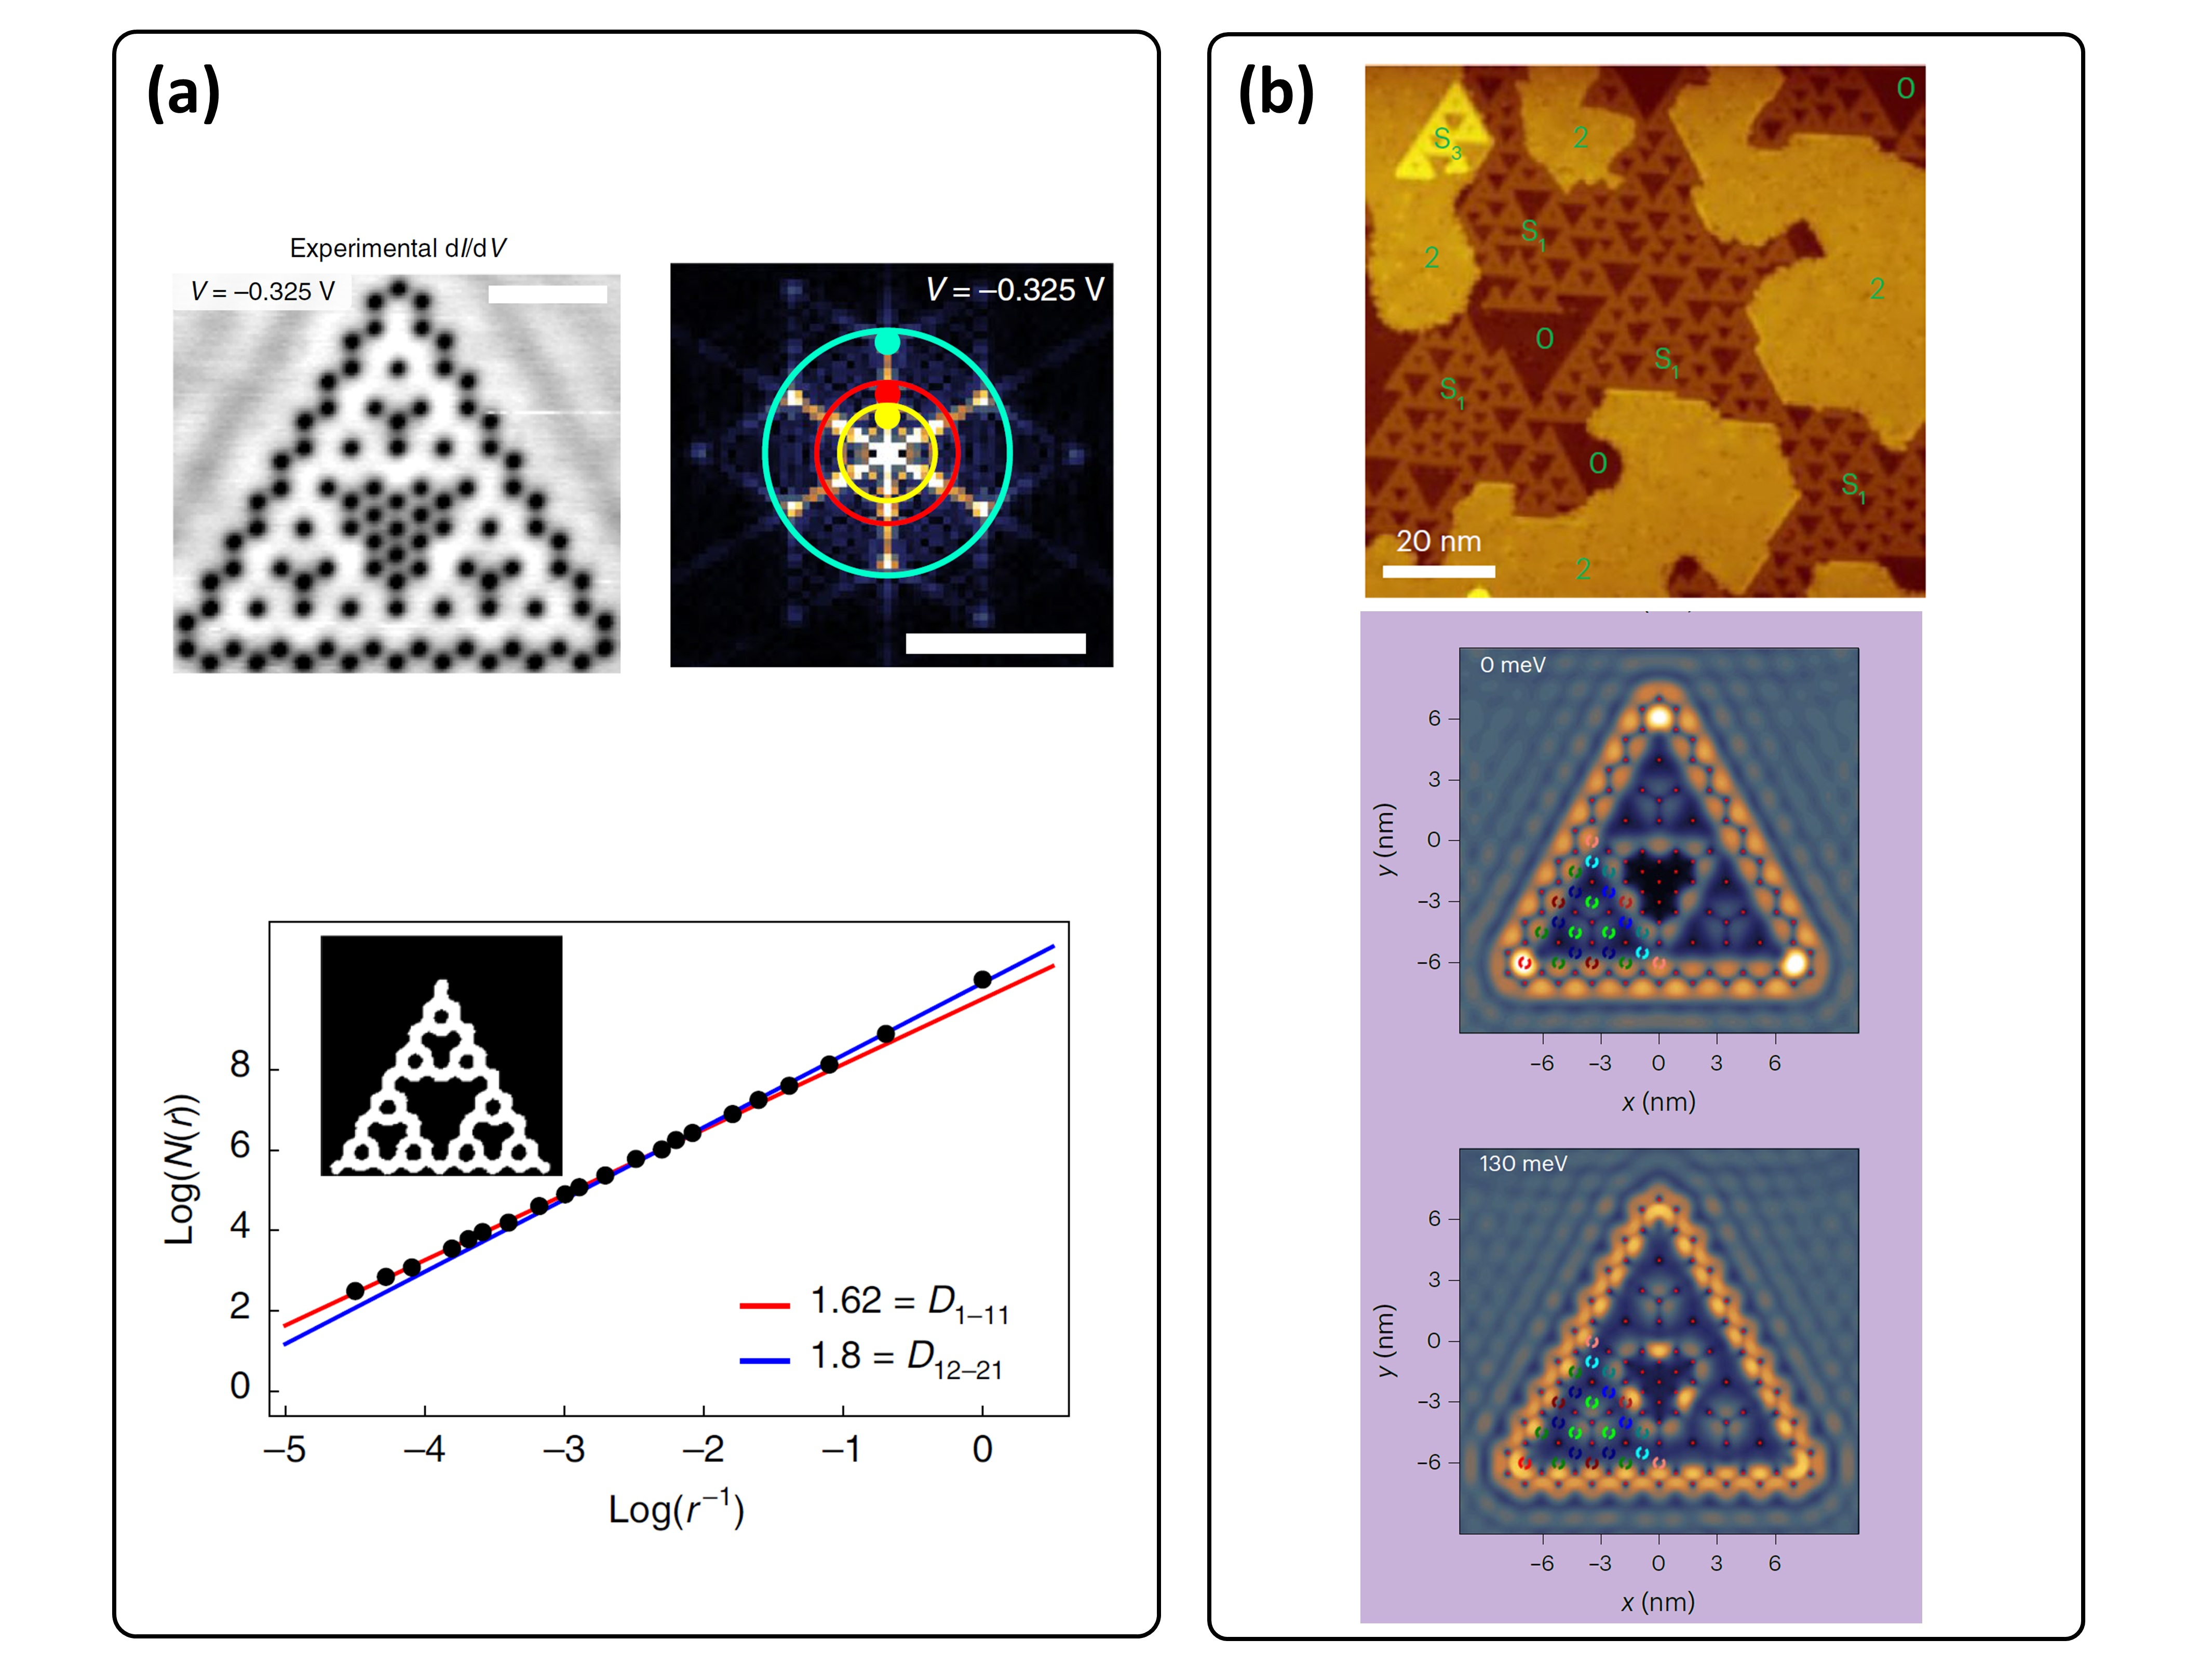
\includegraphics[width=0.75\linewidth]{FractalTopo/ElecFractal.jpg}
    \caption{电子系统分形拓扑绝缘体}
    \label{fig:ElecFractal}
\end{figure}
2021年出现了在电子系统对分形拓扑绝缘体的直接尝试\cite{liu2021sierpinski}。这篇工作报道了在InSb(111)B表面上沉积铋(Bi)薄膜时,观察到了谢尔宾斯基三角形结构。作者发现谢尔宾斯基三角形中没有发生拓扑现象。2023年,该研究团队与文献\cite{kempkes2019design}的团队成功实现了电子系统中的分形拓扑绝缘体。如图\ref{fig:ElecFractal}(b)所示,作者通过将铋薄膜沉积在锑化铟(InSb)基底上形成谢尔宾斯基三角形分形结构。通过扫描隧道显微镜和反射高能电子衍射,作者测量了不同能量下的电子局域态密度(LDOS),发现分形结构中存在零能量的角态和边缘态。

\subsection{光学分形拓扑绝缘体}
最早的光学分形拓扑绝缘体的实验实现出现在2022年\cite{biesenthal2022fractal},文章实现了一个分形Floquet拓扑绝缘体。其采用了谢宾斯基三角形作为分形晶格,光子波导晶格使用激光直写技术制备,拓扑相变通过螺旋波导的Floquet调制产生。传统观点认为,体态是拓扑绝缘体的关键,因为拓扑不变量通常定义在体态中。然而,本文研究了基于精确分形结构谢宾斯基三角形的拓扑绝缘体,如图\ref{fig:PhotonFractal}(a)所示,由于分形的内部空缺,这个晶格的所有格点都是“边”(edge),不存在“体”(bulk)。这篇工作展示了在缺乏传统“体”的情况下,分形结构仍然可以支持拓扑保护的边缘态。这些边缘态不仅存在于外边缘,还存在于分形结构内部的多个层次边缘中。此外,边缘态在分形结构中的传输速度比传统的蜂窝晶格更快。实验还展示了分形和蜂窝晶格混合结构中的拓扑边缘态,证明了两种结构边缘态的兼容性。
\begin{figure}[htbp]
    \centering
    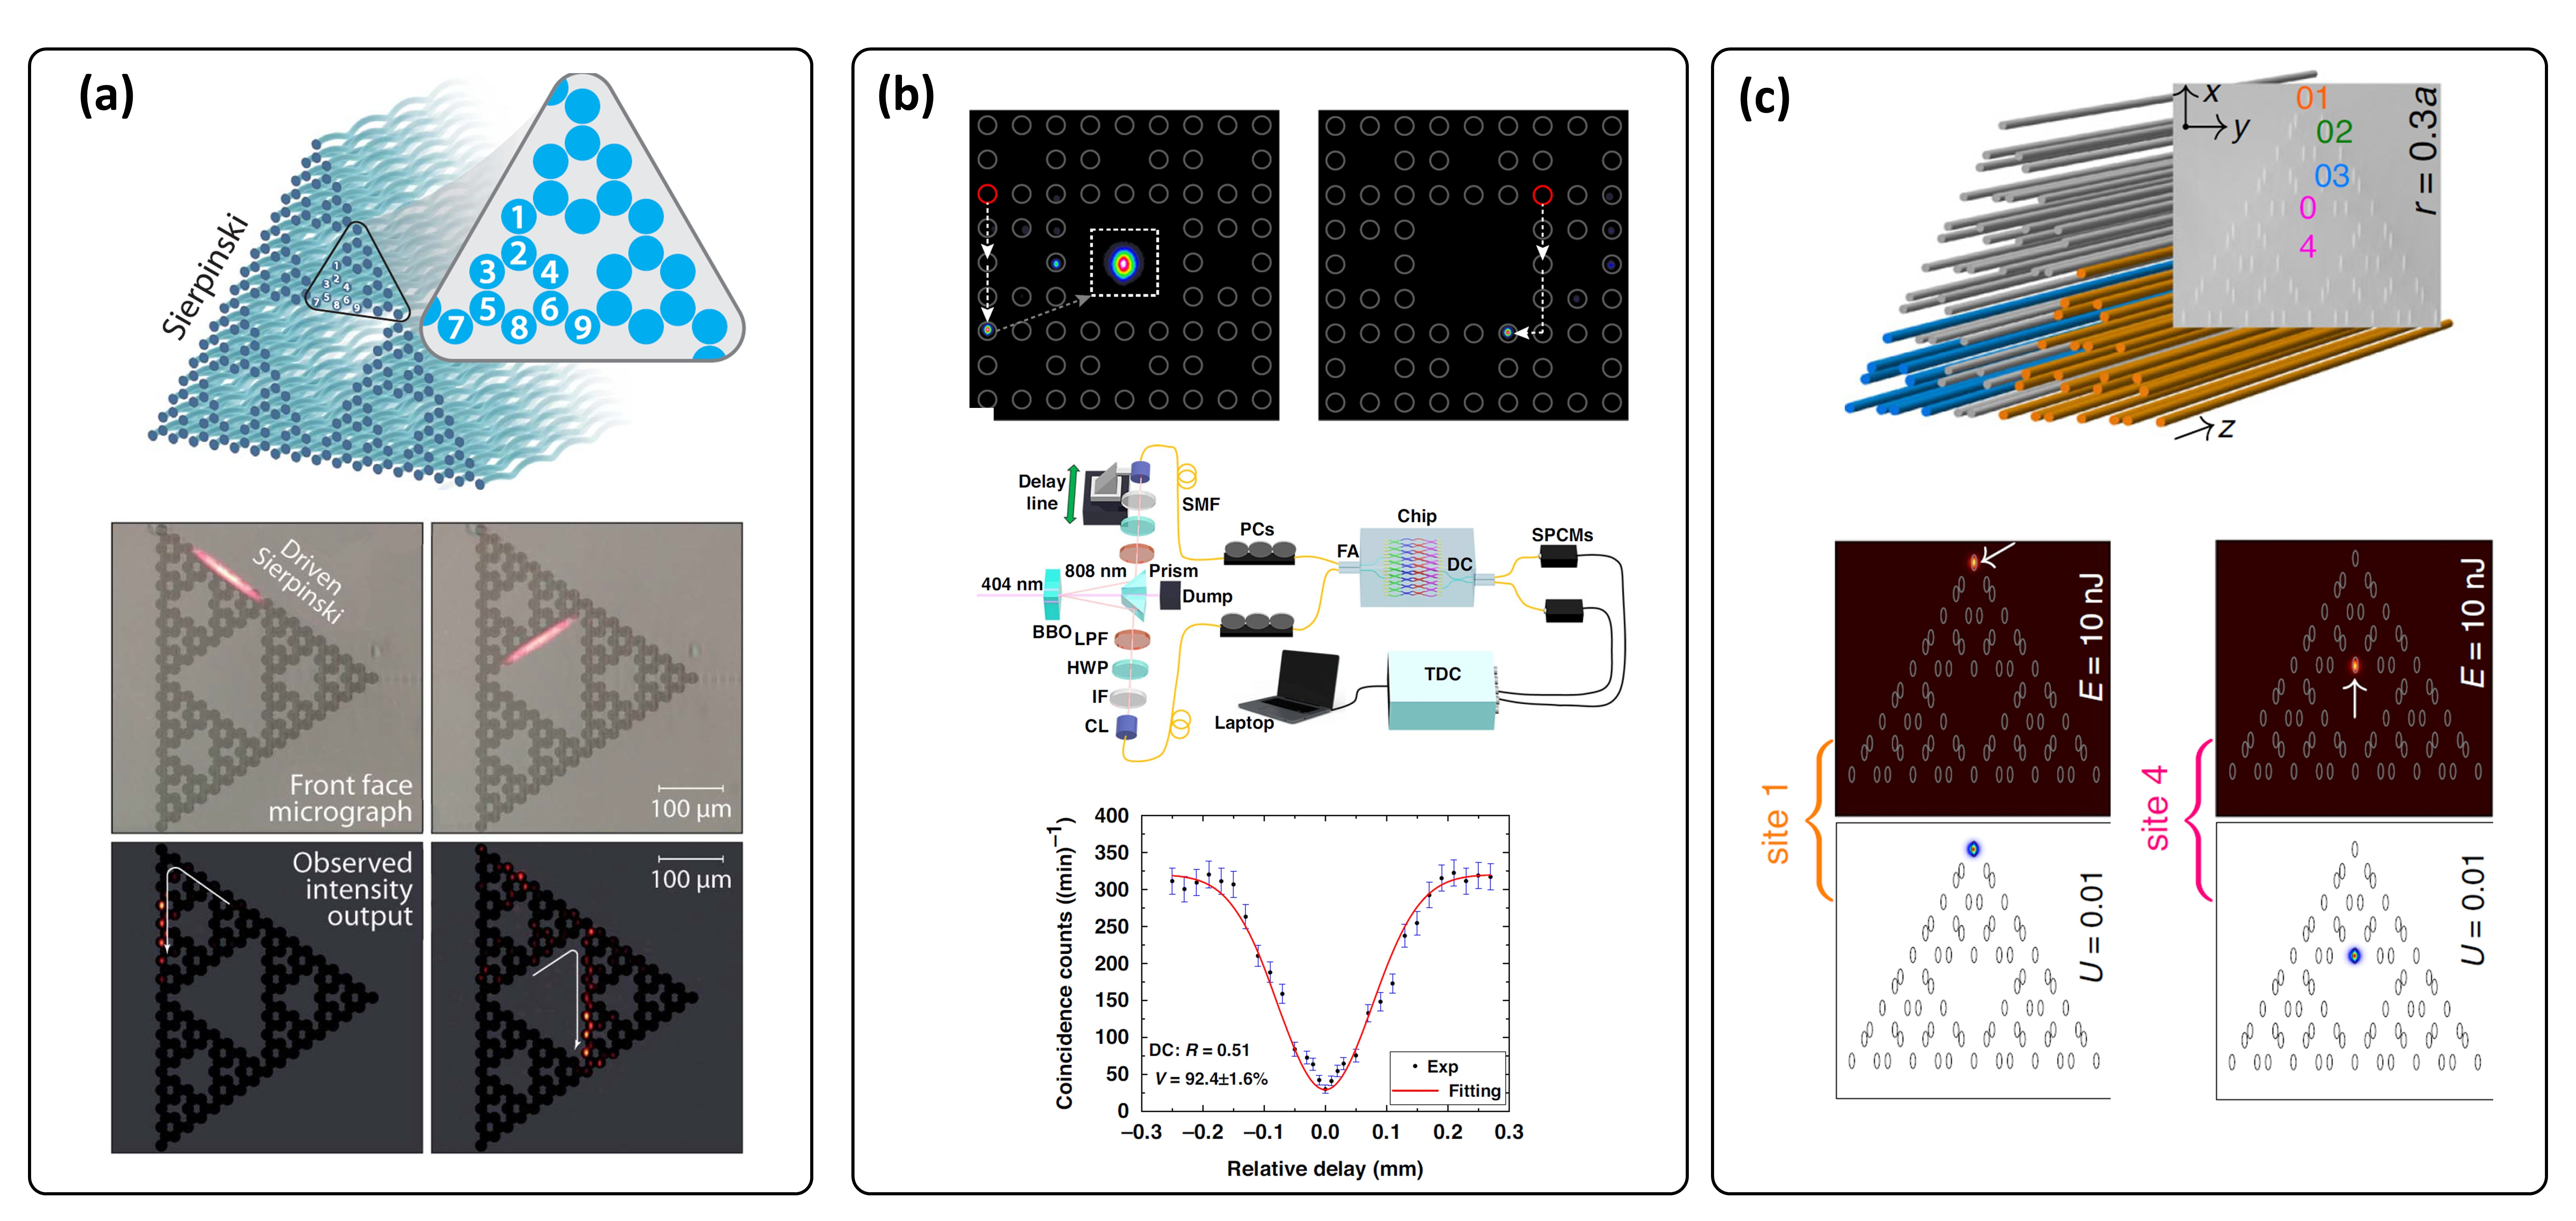
\includegraphics[width=1\linewidth]{FractalTopo/PhotonFractal.jpg}
    \caption{光学分形拓扑绝缘体}(a)分形光学Floquet拓扑绝缘体。上图为螺旋波导管晶格。下图为实验结果。(b)分形光学反常Floquet拓扑绝缘体。上图为单点激发的边缘态传输。中间为单光子边缘态光路图。下图为关联函数测量结果。(c)非线性光学分形高阶拓扑绝缘体。上图为晶格结构。下图为实验结果。图片来源于文献\cite{biesenthal2022fractal,li2023fractal,zhong2024observation}
    \label{fig:PhotonFractal}
\end{figure}
很快分形光子晶体被拓展到反常Floquet系统\cite{li2023fractal}。尽管反常Floquet拓扑绝缘体的标准拓扑不变量(如陈数)为零,但其具有非零的绕数,支持拓扑边缘态。然而,现有的反常Floquet拓扑绝缘体通常只支持一种手性边缘态,难以应用于多态拓扑量子系统。分形拓扑绝缘体由于其自相似性和非整数维度,具有更少波导的分形光子反常Floquet拓扑绝缘体支持比二维晶格多得多的手性边缘模式,如图\ref{fig:PhotonFractal}(b)所示。此外实验生成了多个单光子手性边缘态,并观察到了高可见度(超过$90\%$)的量子干涉。

光学分形拓扑绝缘体的实验观测不仅局限于线性体系,最近有工作实现了在非线性高阶系统的光学分形拓扑绝缘体\cite{zhong2024observation}。实验观察到了从拓扑角态分岔出的无阈值空间孤子,并展示了通过输入光束功率可以有效控制这些孤子的局域化,见图\ref{fig:PhotonFractal}(c)。分形高阶拓扑绝缘体中的非线性孤子表现出独特的局域化行为,在外角和多个内角处的光局域化表现出显著差异。

\subsection{其他分形拓扑绝缘体}
分形拓扑绝缘体的概念不仅在电子和光子系统中引发了广泛的研究兴趣,也在声学系统和弹性波系统中得到了实现和深入探索。研究人员通过设计具有分形结构的声学材料,成功实现了陈绝缘体\cite{li2023fractality}、高阶拓扑相\cite{LI20222040}以及自旋陈绝缘体\cite{lai2024spin}等拓扑态,并在声学系统中展开了丰富多样的研究。此外,研究人员还在弹性波系统中对分形高阶拓扑相的实现和性质进行了深入的探讨\cite{ma2023elastic,dorin2024uncovering}。

